\pdfoutput=1
\documentclass[sigconf,anonymous,review]{acmart}

% Suppress ACM metadata for workshop submission draft
\settopmatter{printacmref=false}
\renewcommand\footnotetextcopyrightpermission[1]{}
\acmConference[HotCarbon '26]{Workshop on Sustainable Computer Systems}{July 16--17, 2026}{Seattle, WA, USA}
\acmYear{2026}

\usepackage{booktabs}
\usepackage{multirow}
\usepackage{xcolor}
\usepackage{siunitx}
\usepackage{amsmath}

\sisetup{group-separator={,}, group-minimum-digits=4}

% Allow line breaks in the long env-var name
\newcommand{\perfboost}{\texttt{CUDA\_\hspace{0pt}DISABLE\_\hspace{0pt}PERF\_\hspace{0pt}BOOST}}

\begin{document}

\title{The Model Parking Tax: Quantifying the Hidden Energy Cost of Always-On GPU Model Deployment}

\author{Anonymous}
\affiliation{
    \institution{Anonymous Institution}
}

\begin{abstract}
The AI inference industry keeps models loaded in GPU memory around the clock to avoid cold-start latency, treating idle power as a fixed cost of readiness. We show this cost has the wrong shape. Combining 18~days of production telemetry (\num{335267} samples, 14~H100 GPUs) with controlled dose-response experiments on H100 (HBM3), A100 (HBM2e), and L40S (GDDR6), we find that idle power is piecewise constant in CUDA context, not VRAM: creating a context forces a DVFS transition costing $+26$--$66$\,W, while the marginal effect of allocated memory is below $0.02$\,W/GB on every device. Model size, in other words, is the wrong variable to optimize. NVIDIA's \perfboost flag reduces idle-with-context power to bare-idle levels on tested systems (Hopper $-$55\,W, Ampere $-$10.6\,W of 11.1\,W overhead) with no steady-state latency penalty under vLLM. The tax scales linearly at ${\sim}52$\,W per H100 across tensor, data, and mixed parallelism, and the cold-start ramp does not compound with GPU count. At industry scale, the anomaly wastes an estimated 92--1{,}745\,GWh/year---a fix waiting on a one-line environment variable.
\end{abstract}

\keywords{GPU energy, idle power, DVFS, CUDA, model serving, sustainability}

\maketitle

% ===========================================================================
\section{Introduction}
% ===========================================================================

The default operating model for AI inference is to keep models loaded in VRAM indefinitely, accepting continuous idle power to avoid cold-start latency. Cold-start optimization is well-studied~\cite{serverlessllm,nvidia-streamer,hydraserve,lambdascale}, but the \emph{ongoing energy cost of readiness} has been treated as an unquantified constant. The 2024 US Data Center Energy Usage Report estimates GPU idle power at $\sim$20\% of TDP~\cite{doe-report}. Patel et al.~\cite{patel-cal23} showed that CUDA contexts on A100 GPUs force higher clock frequencies even at 0\% utilization. Concurrent work by Lei et al.~\cite{lei-idle} characterizes the prevalence of execution-idle (19.7\% of in-execution time across 756~GPUs); we focus instead on the underlying mechanism.

No prior work has measured the marginal idle energy cost \emph{per GB of VRAM}, tested the result across GPU architectures and memory technologies, or evaluated vendor-provided mitigations. We fill this gap with three studies:

\begin{enumerate}
    \item \textbf{Production telemetry}: \num{335267} samples from 14~H100 GPUs over 18~days.
    \item \textbf{Controlled experiments}: Dose-response on H100 (HBM3), A100 (HBM2e), and L40S (GDDR6), varying VRAM from 0 to 40--72\,GB.
    \item \textbf{Multi-GPU scaling}: 9~conditions on a 4$\times$H100 node testing tensor parallelism (TP), data parallelism (DP), and mixed configurations with and without \perfboost.
\end{enumerate}

Our central finding is that idle power follows:
\begin{equation}
    P_{\text{idle}}(C, V) = P_{\text{base}} + \Delta P_{\text{DVFS}} \cdot \mathbf{1}_{[C=1]} + \beta V
    \label{eq:model}
\end{equation}
where $C \in \{0,1\}$ indicates whether a CUDA context is active, $V$ is VRAM occupancy in GB, $P_{\text{base}}$ is bare-idle power (no context), $\Delta P_{\text{DVFS}}$ is the clock-boost overhead triggered by the context, and $\beta$ is the marginal VRAM slope. We find $|\beta| < 0.02$\,W/GB on all devices---the optimization priority is $\partial P / \partial C \gg \partial P / \partial V$.

% ===========================================================================
\section{Background}
% ===========================================================================

\paragraph{DVFS anomaly.} NVIDIA datacenter GPUs support Dynamic Voltage and Frequency Scaling (DVFS). Without a CUDA context, Streaming Multiprocessor (SM) clocks idle at 210--345\,MHz. Once a CUDA context is created, the SM clock jumps to maximum boost and \emph{remains there} at 0\% utilization~\cite{patel-cal23}---converting a variable cost into a fixed cost decoupled from both utilization and memory occupancy.

\paragraph{Memory physics predicts $\beta \approx 0$.} GPU memory power decomposes into background, refresh, and activation components~\cite{hbm-spec,micron-ddr}. Background power is constant; refresh sweeps all rows per JEDEC specification regardless of occupancy; activation is zero at idle. Therefore $\partial P_{\text{mem}} / \partial \text{occupancy} \approx 0$---a prediction from DRAM physics that our experiments validate across HBM3, HBM2e, and GDDR6.

% ===========================================================================
\section{Related Work}
% ===========================================================================

Patel et al.~\cite{patel-cal23} first observed that idle-but-allocated A100 GPUs lock SM clocks at maximum boost, adding ${\sim}20$\,W above bare idle. They did not vary VRAM occupancy, test other architectures, or evaluate mitigations. Patel et al.~\cite{patel-asplos24} later characterized LLM inference power phases in the cloud but focused on active workloads. Zeus~\cite{zeus} optimized GPU energy for \emph{active} DNN training via frequency scaling. Burtscher et al.~\cite{burtscher-power} showed \texttt{nvidia-smi} samples power for only ${\sim}25$\% of runtime---a measurement caveat we address with long steady-state windows ($n=40$, 20\,min/phase).

Concurrent work by Lei et al.~\cite{lei-idle} characterizes ``execution-idle'' via 31-day passive telemetry on a 756-GPU cluster, finding 19.7\% of in-execution time is idle. Their frequency-downscaling mitigation saves 22--34\% with persistent latency tradeoffs. Our work is complementary: they quantify \emph{how often} execution-idle occurs at scale; we isolate \emph{why} (CUDA context, not VRAM) via controlled experiments and show the \perfboost flag achieves comparable savings with only a transient cost.

Several systems reduce cold-start latency~\cite{serverlessllm,nvidia-streamer,hydraserve,lambdascale} but do not address the idle power of models that remain loaded.

% ===========================================================================
\section{Methodology}
% ===========================================================================

\paragraph{Phase~1: Production telemetry.} We instrumented 14~H100 80GB SXM5 GPUs across 2~Kubernetes nodes, collecting \num{335267} idle-state samples (0\% utilization) over 18~days via NVIDIA's Data Center GPU Manager (DCGM)/Prometheus at 30\,s intervals. VRAM ranged from 3\,MB to 79\,GB.

\paragraph{Phase~2: Controlled experiments.} Within-subject dose-response on three GPUs (Table~\ref{tab:cross}). Protocol: bare-idle baseline, create CUDA context, sequentially allocate increasing VRAM via \texttt{torch.empty}, record \texttt{nvidia-smi} every 30\,s for 20\,min per level ($n=40$/phase). Validated with real model weights (Qwen2.5-7B~\cite{qwen2} fp16) on all three architectures ($<$0.5\,W difference from empty tensors). We apply Two One-Sided Tests (TOST)~\cite{schuirmann-tost} with $\Delta = \pm 0.1$\,W/GB to formally bound the VRAM effect.

\paragraph{Phase~3: Multi-GPU} 9~conditions on a 4$\times$H100 SXM node (NVLink, driver 580.126.09) using vLLM~\cite{vllm} serving Qwen2.5-7B: bare idle, TP=2/4, DP=2, TP2$\times$DP2, each with and without \perfboost. Per condition: warm latency ($n=50$), DVFS decay (5\,min at 1\,s), idle power ($n=40$, 20\,min), and cold-start ramp (60\,s soak).

% ===========================================================================
\section{Results}
% ===========================================================================

\subsection{The Parking Tax Is a Step Function}

\paragraph{Production telemetry.} Phase~1 reveals a bimodal distribution: bare idle (345\,MHz, 74.7\,W) vs.\ CUDA-active (1980\,MHz, 145.5\,W). The context effect is $+70.9$\,W ($d = 7.3$). Within CUDA-active GPUs, regression across 3.2--77.1\,GB yields slope $= 0.013$\,W/GB ($R^2 = 0.001$).

\paragraph{Cross-architecture dose-response.} Table~\ref{tab:cross} presents the controlled results. On all three GPUs, CUDA context creation triggers a discrete DVFS step ($+26$--$66$\,W) while varying VRAM from 0 to 40--72\,GB changes power by $<$1\,W. TOST rejects $|\beta| \geq 0.1$\,W/GB on all devices ($p < 0.05$). The parking tax is $>$99\% attributable to the CUDA context on every architecture---consistent across HBM3, HBM2e, and GDDR6 (Figure~\ref{fig:hero}).

\begin{table}[t]
\caption{Cross-architecture parking tax. $\beta$ is the VRAM regression slope across CUDA-active phases. All GPUs at 0\% utilization.}
\label{tab:cross}
\small
\begin{tabular}{lrrr}
\toprule
 & \textbf{H100} & \textbf{A100} & \textbf{L40S} \\
 & \textbf{(HBM3)} & \textbf{(HBM2e)} & \textbf{(GDDR6)} \\
\midrule
Bare idle (W) & 71.8 & 53.7 & 35.6 \\
CUDA ctx power (W) & 121.7 & 80.0 & 102.1 \\
\textbf{Context overhead (W)} & \textbf{+49.9} & \textbf{+26.3} & \textbf{+66.4} \\
Context (\% of TDP) & 7.1\% & 8.8\% & 19.0\% \\
\midrule
$\beta$ (W/GB) & $-$0.002 & $-$0.001 & $-$0.002 \\
$p_{\text{TOST}}$ ($|\beta| < 0.1$) & $10^{-9}$ & $<0.001$ & $<0.05$ \\
\textbf{Context \% of tax} & \textbf{$>$99\%} & \textbf{$>$99\%} & \textbf{$>$99\%} \\
\bottomrule
\end{tabular}
\end{table}

\begin{figure}[t]
    \centering
    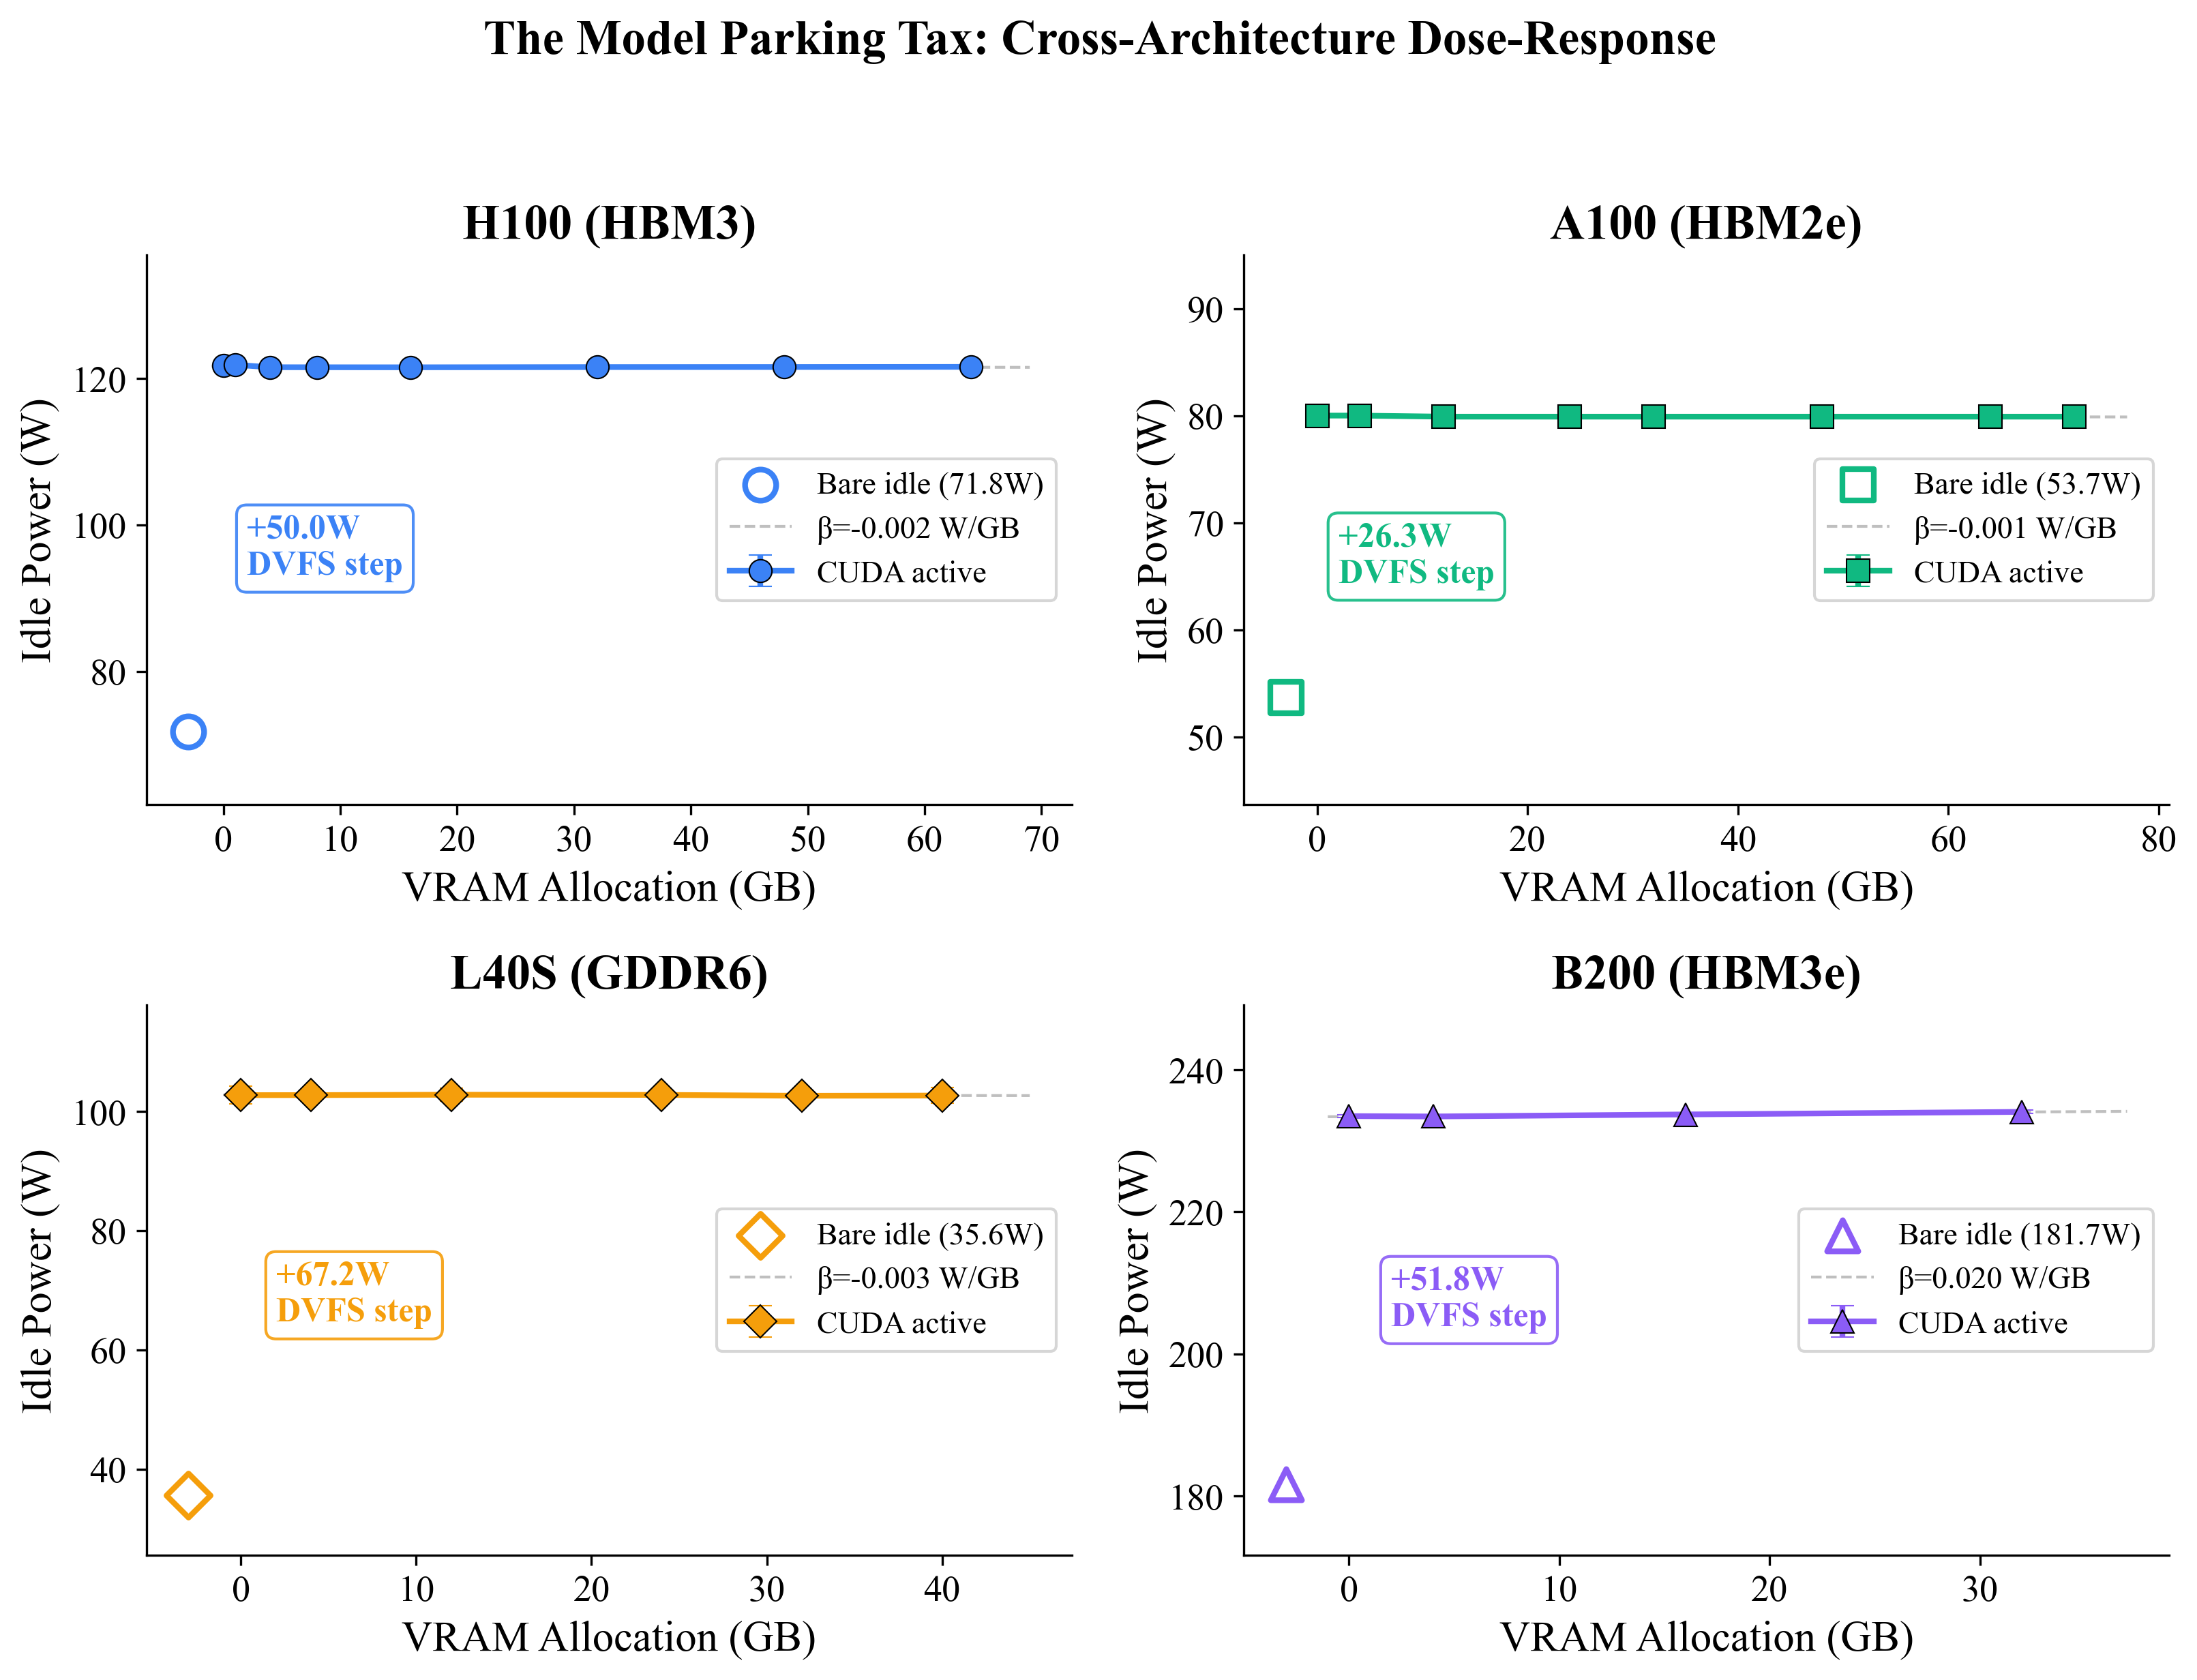
\includegraphics[width=\columnwidth]{cross_architecture_dose_response.png}
    \caption{The parking tax across three architectures. Large markers: bare-idle (no CUDA context). Connected lines: CUDA-active phases with increasing VRAM. The DVFS step dominates; all dose-response curves are flat across HBM3, HBM2e, and GDDR6.}
    \label{fig:hero}
\end{figure}

\subsection{Vendor Mitigation: \perfboost}

NVIDIA shipped \perfboost in driver 580.105.08 (November 2025) to suppress idle-context clock boosting. Table~\ref{tab:flag} shows the results.

\begin{table}[t]
\caption{Effect of \perfboost on idle power and inference latency. Idle: $n=40$, 20-min phases. Latency: $n=50$ warm requests (128-tok prompt/completion). Cold: first request after 60\,s idle.}
\label{tab:flag}
\small
\begin{tabular}{@{}lrrrr@{}}
\toprule
 & \multicolumn{2}{c}{\textbf{H100 SXM}} & \multicolumn{2}{c}{\textbf{A100 SXM4}} \\
\cmidrule(lr){2-3} \cmidrule(lr){4-5}
 & \textbf{Base} & \textbf{Flag} & \textbf{Base} & \textbf{Flag} \\
\midrule
Idle power (W) & 128.1 & 73.1 & 75.1 & 64.5 \\
SM clock (MHz) & 1980 & 345 & 1155 & 210 \\
Tax recovered & --- & $>$99\% & --- & 96\% \\
\midrule
vLLM idle (W) & 128.6 & 73.1 & 73.9 & 64.3 \\
Warm latency (ms) & 533.4 & 533.3 & 910.0 & 910.0 \\
Cold req\,1 (ms) & 546 & 683 & 921 & 1130 \\
Ramp penalty & +10 & +147 & +11 & +220 \\
\bottomrule
\end{tabular}
\end{table}

On the H100, the flag reduces idle-with-context power to bare-idle levels: idle power drops from 128.1\,W to 73.1\,W (indistinguishable from bare idle at 73.3\,W). The 1.5\,W difference from the Phase~2 H100 baseline (71.8\,W, Table~\ref{tab:cross}) reflects inter-session variance consistent with the ${\sim}23$\,W inter-device spread observed in Phase~1. On the A100, it recovers 96\% of the 11.1\,W overhead. Through vLLM serving Qwen2.5-7B, steady-state latency is identical at all percentiles through p99 on both architectures---CUDA graphs function correctly under the flag. The only cost is a one-time DVFS ramp on the first request after idle ($+$147\,ms H100, $+$220\,ms A100), gone by request~2 and mitigable with a warmup probe. Figure~\ref{fig:perf-boost-power} shows the effect visually.

\begin{figure}[t]
    \centering
    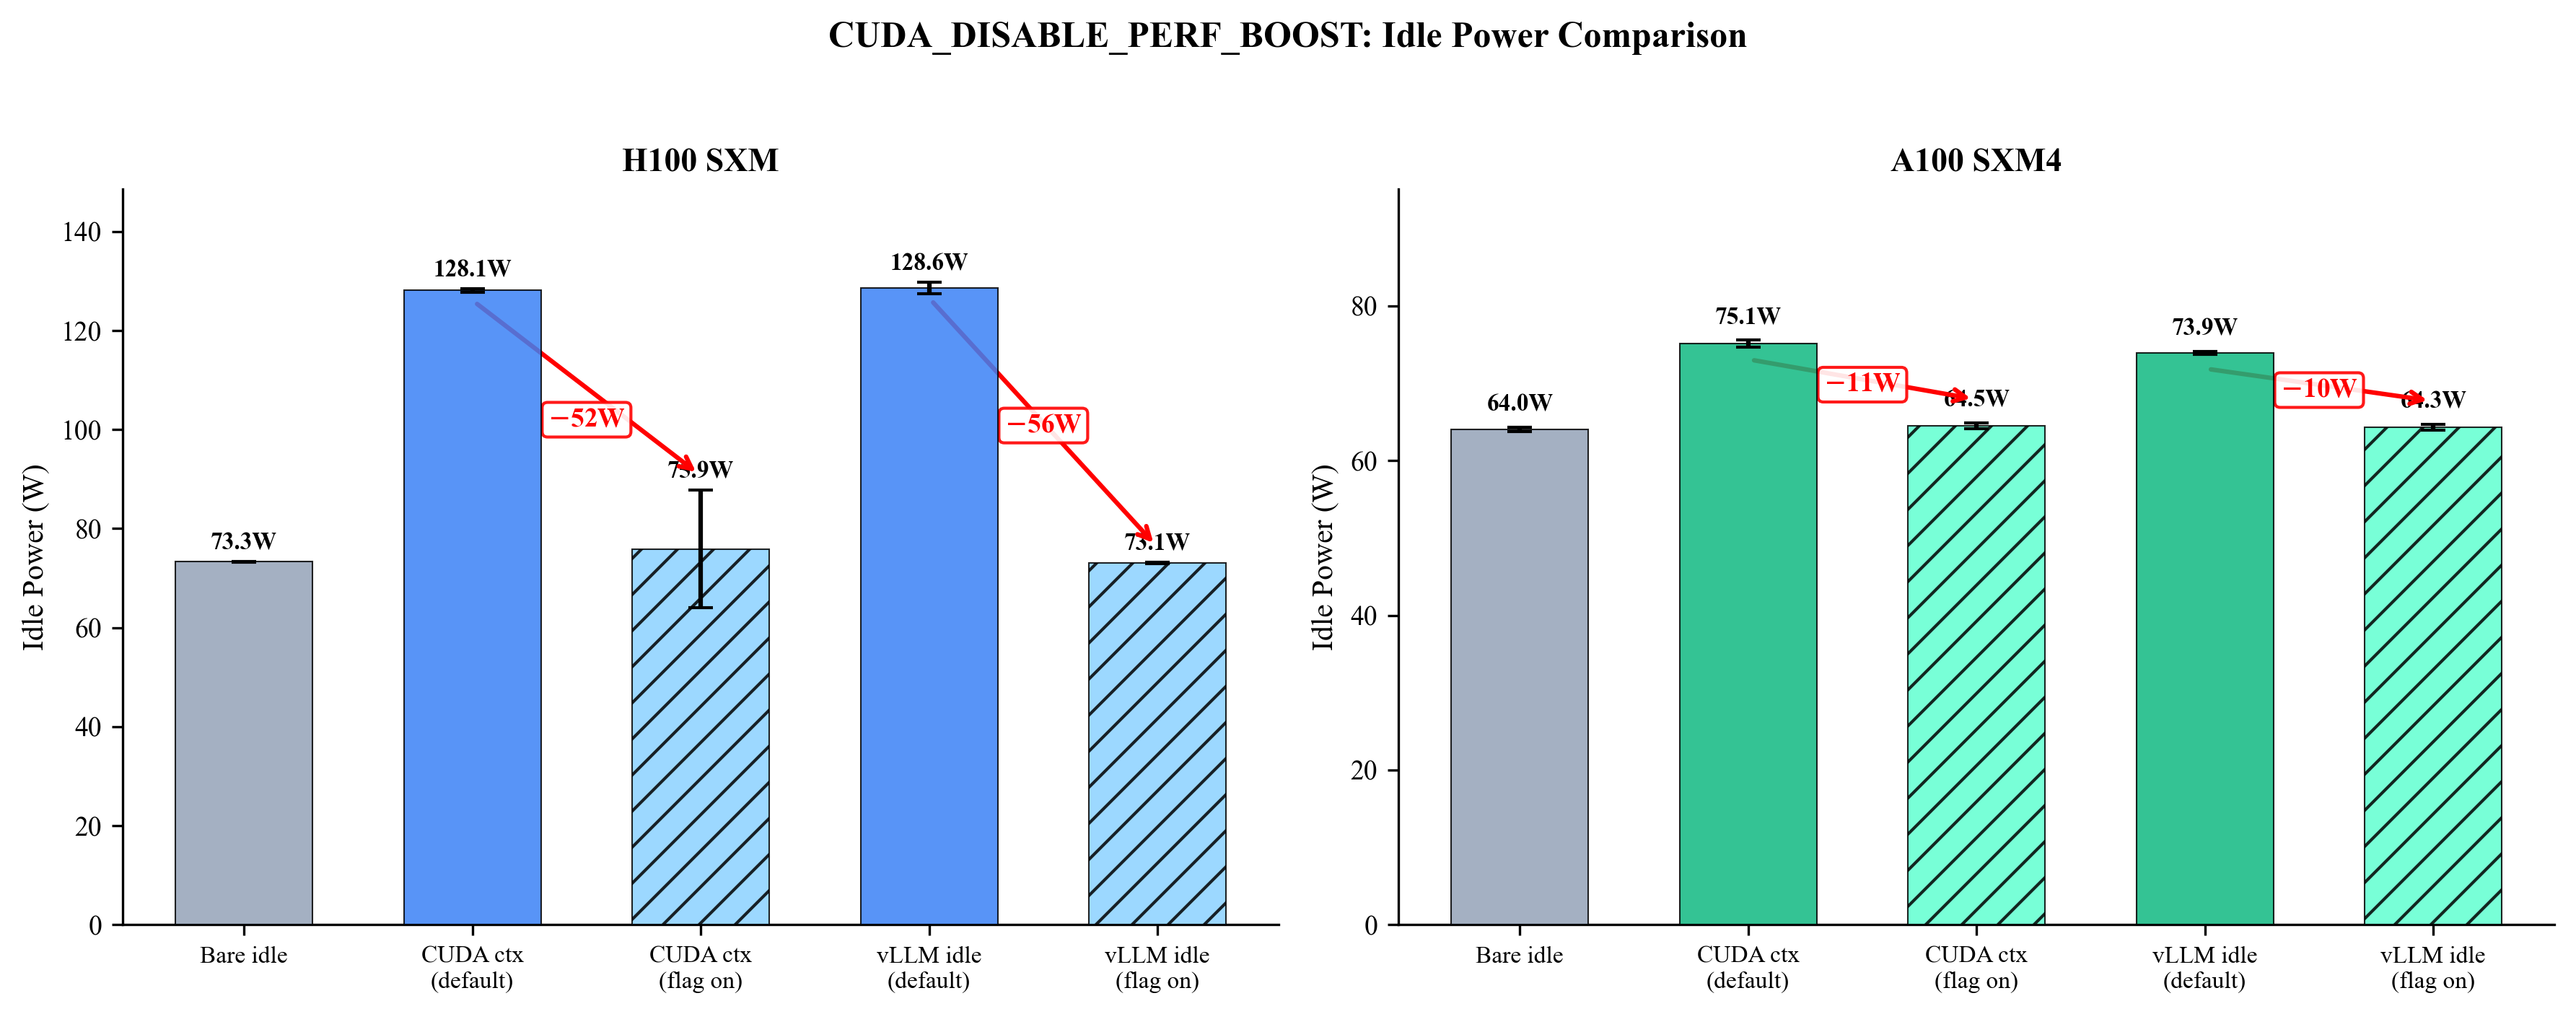
\includegraphics[width=\columnwidth]{perf_boost_power_comparison.png}
    \caption{Effect of \perfboost on idle power. Hatched bars: flag enabled. On both H100 and A100, the flag reduces idle-with-context power to bare-idle levels whether the context comes from \texttt{torch.empty} or a full vLLM stack.}
    \label{fig:perf-boost-power}
\end{figure}

\subsection{Multi-GPU Scaling}

On the 4$\times$H100 node, the parking tax is ${\sim}52$\,W/GPU across all parallelism strategies (Table~\ref{tab:multi-gpu})---matching the single-GPU measurement. The communication pattern (NVIDIA Collective Communications Library (NCCL) all-reduce for TP, independent contexts for DP) does not matter: the tax scales linearly as $P_{\text{park}}(N) = N \times 52$\,W. The flag eliminates the tax under all configurations (per-GPU idle within 0.6\,W of bare idle). Cold-start penalty does not compound with $N$: all configurations show $+$145--176\,ms, matching the single-GPU baseline, because NCCL barriers synchronize all GPUs to ramp in parallel. With the flag enabled, clocks drop to bare idle within 2\,s of the last request and recover on the next (Figure~\ref{fig:decay-curve}).

\begin{table}[t]
\caption{Multi-GPU parking tax (4$\times$H100 SXM, Qwen2.5-7B fp16). Tax: per-GPU overhead vs.\ bare idle (71.7\,W). Cold penalty: first request after 60\,s idle minus recovery mean.}
\label{tab:multi-gpu}
\small
\begin{tabular}{@{}lrrrr@{}}
\toprule
\textbf{Condition} & \makebox[3em][r]{\textbf{Per-GPU}} & \makebox[3em][r]{\textbf{Tax/}} & \makebox[3.5em][r]{\textbf{Warm}} & \makebox[3.5em][r]{\textbf{Cold}} \\
 & \makebox[3em][r]{\textbf{(W)}} & \makebox[3em][r]{\textbf{GPU}} & \makebox[3.5em][r]{\textbf{(ms)}} & \makebox[3.5em][r]{\textbf{pen.}} \\
\midrule
TP=4 baseline & 125.6 & $+$53.9 & 237.7 & $+$13.8 \\
TP=4 flag on & 71.8 & $+$0.1 & 250.6 & $+$156.5 \\
TP2$\times$DP2 base & 125.8 & $+$54.1 & 352.9 & $+$7.2 \\
TP2$\times$DP2 flag & 72.3 & $+$0.6 & 353.1 & $+$144.9 \\
\bottomrule
\end{tabular}
\end{table}

\begin{figure}[t]
    \centering
    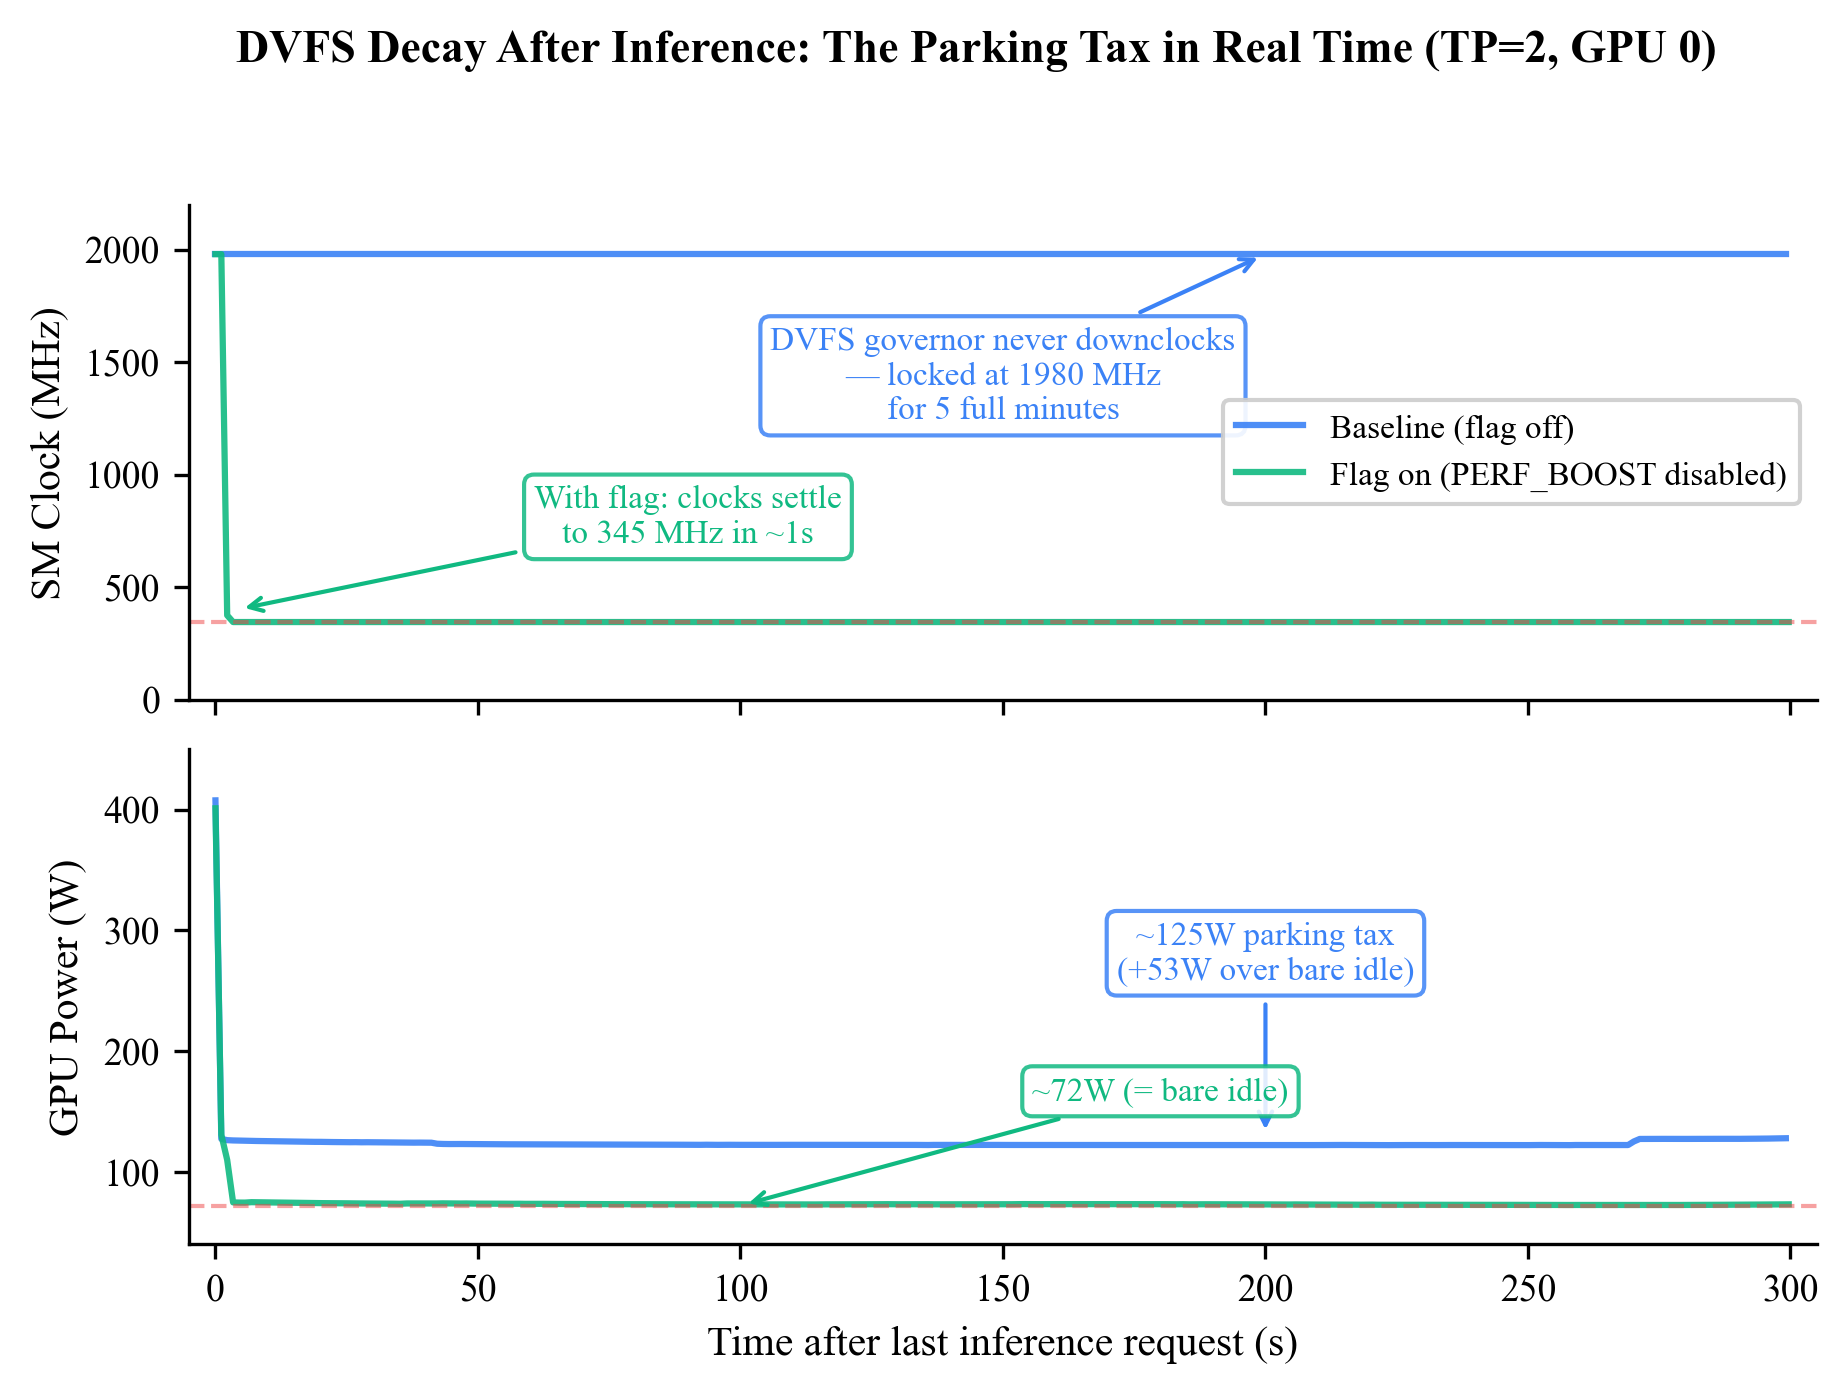
\includegraphics[width=\columnwidth]{multi_gpu_decay_curve.png}
    \caption{DVFS decay after last request (TP=2, GPU~0). Without the flag, clocks remain locked at 1980\,MHz indefinitely. With the flag, clocks drop to 345\,MHz within 2\,s and power transitions to bare idle in $<$4\,s.}
    \label{fig:decay-curve}
\end{figure}

\subsection{Cold-Start Breakeven}
\label{sec:breakeven}

If the flag is unavailable (older drivers, non-NVIDIA hardware), the alternative is to evict the model and cold-start on the next request. The energy breakeven between keeping warm and cold-starting is:
\begin{equation}
    T^* = \frac{P_{\text{load}} \cdot t_{\text{load}}}{P_{\text{park}}}
    \label{eq:breakeven}
\end{equation}
where $P_{\text{load}}$ is the mean power during loading, $t_{\text{load}}$ is the loading duration, and $P_{\text{park}}$ is the idle-context overhead from Equation~\ref{eq:model}. Table~\ref{tab:breakeven} shows breakeven intervals for the H100 ($P_{\text{park}} = 49.9$\,W). For standard PyTorch loading of a 70B model (45\,s, ${\sim}300$\,W), $T^* \approx 4.5$\,min---any idle period longer than this wastes more energy than a cold start. Faster loaders shrink $T^*$: ServerlessLLM (70B) brings it to 48\,s, and NVIDIA's Model Streamer (8B) to 20\,s---model sizes differ, but both illustrate how loader optimization shifts the breakeven. On the A100 ($P_{\text{park}} = 26.3$\,W), $T^*$ roughly doubles; on the L40S ($P_{\text{park}} = 66.4$\,W), it shrinks by ${\sim}25$\%.

\begin{table}[t]
\caption{Cold-start energy breakeven on H100 ($P_{\text{park}} = 49.9$\,W). $T^*$: idle duration beyond which eviction saves energy.}
\label{tab:breakeven}
\small
\begin{tabular}{@{}lrrr@{}}
\toprule
\textbf{Loading method} & \makebox[3em][r]{$P_{\text{load}}$} & \makebox[3em][r]{$t_{\text{load}}$} & \makebox[3em][r]{$T^*$} \\
 & \makebox[3em][r]{(W)} & \makebox[3em][r]{(s)} & \\
\midrule
Qwen2.5-7B (measured) & 124 & 30 & 1.2\,min \\
PyTorch 70B (est.) & 300 & 45 & 4.5\,min \\
ServerlessLLM 70B~\cite{serverlessllm} & 300 & 8 & 48\,s \\
Model Streamer 8B~\cite{nvidia-streamer} & 200 & 5 & 20\,s \\
\bottomrule
\end{tabular}
\end{table}

If requests arrive as a Poisson process with rate $\lambda$, the optimal eviction threshold is $\lambda^* = P_{\text{park}} / (P_{\text{load}} \cdot t_{\text{load}})$; for H100 with PyTorch loading, $\lambda^* \approx 13$\,req/hr. The \perfboost flag reframes this tradeoff: it eliminates the parking tax while keeping the model loaded, replacing the cold-start cost with a transient ${\sim}150$\,ms ramp. Where the flag is available, eviction is unnecessary unless VRAM must be reclaimed for other models.

\subsection{Industry-Scale Impact}

Three indicative inputs: 3.76M datacenter GPUs shipped in 2023~\cite{nvidia-shipments}, 35\% idle~\cite{flexera}, and $\bar{P}_{\text{park}} = 40$\,W fleet-weighted average. Under these assumptions, the CUDA context overhead wastes an estimated ${\sim}462$\,GWh/year (sensitivity: 92--1{,}745\,GWh/year). Even the conservative bound exceeds a small city's annual consumption.

% ===========================================================================
\section{Discussion}
% ===========================================================================

\paragraph{Prescription.} Based on our measurements, setting \perfboost\texttt{=1} in the process environment before launching the inference server appears to be the cheapest available mitigation. The flag is read at CUDA context creation. While serving: full boost, no latency penalty. While idle: clocks drop to bare idle within 2\,s automatically (Figure~\ref{fig:decay-curve}). On next request: ${\sim}150$\,ms one-time ramp, constant regardless of GPU count. A 4-GPU node saves ${\sim}215$\,W; a 1{,}000-GPU cluster at 30\% idle saves ${\sim}16$\,kW (${\sim}140$\,MWh/year).

\paragraph{Pipeline parallelism and multi-node.} Our experiments cover TP and DP on a single NVLink node. Two natural extrapolations follow. Pipeline parallelism (PP)---does the tax behave the same when stages communicate via point-to-point send/recv rather than all-reduce? The mechanism we identify is per-CUDA-context and independent of communication pattern, which suggests yes, but we have not measured it directly. Multi-node deployments---the DVFS governor responds to local SM activity, not the interconnect fabric, so InfiniBand or RDMA over Converged Ethernet (RoCE) should not change the per-GPU result. Under this hypothesis, a 64-GPU deployment across 8 nodes would waste $64 \times 52 \approx 3{,}328$\,W idle. Both extrapolations are testable; we leave direct validation as future work.

\paragraph{Adoption barriers.} The flag has been available since driver 580.105.08 (November 2025) but has not seen adoption. Two factors plausibly contribute. First, the flag is undocumented in mainstream inference-serving frameworks---neither vLLM~\cite{vllm}, SGLang, nor TensorRT-LLM expose it as a configuration option, and its interaction with CUDA graphs had not been publicly validated prior to this work. Second, the structure of the inference-serving market splits incentives: engineers configuring inference engines are typically not the engineers paying the power bill, and cloud GPU tenants on flat hourly rates have no visibility into idle power. The cost falls on infrastructure operators---cloud providers, inference companies, on-premise enterprises---who have the incentive to act but lack documentation to change an outdated default. Native support in serving frameworks could close both gaps simultaneously.

\paragraph{Relationship to execution-idle.} Lei et al.~\cite{lei-idle} find 19.7\% of in-execution time is idle across 756~GPUs. Our parking tax is the dominant sub-component when activity is strictly zero. Their frequency-downscaling mitigation achieves 22--34\% savings but with \emph{persistent} latency tradeoffs; the \perfboost flag achieves comparable savings with only a transient cost, which appears preferable for workloads with distinct idle and active phases.

\paragraph{Limitations.} We test one device per architecture in Phase~2 (complemented by 14~H100s in Phase~1). The flag was not tested on L40S. Multi-GPU experiments cover a single 4$\times$H100 node; PP, multi-node, and 8-GPU configurations are untested. We measure one model size (Qwen2.5-7B). A full scheduler evaluation comparing time-to-live (TTL) and breakeven policies under varied traffic patterns is future work.

% ===========================================================================
\section{Conclusion}
% ===========================================================================

The model parking tax---26--66\,W per GPU depending on architecture---is a fixed cost of the CUDA context, not a variable cost of model size. This holds across HBM3, HBM2e, and GDDR6. NVIDIA's \perfboost flag reduces idle-with-context power to bare-idle levels on tested architectures (Hopper, Ampere) with no steady-state latency penalty; the only cost is a transient ${\sim}150$\,ms ramp on the first request after idle. The tax scales linearly with GPU count, and the per-GPU DVFS mechanism is independent of interconnect, suggesting the result extends to pipeline-parallel and multi-node deployments. Setting the flag at process start lets the DVFS governor handle idle-active transitions automatically. Native integration into inference-serving frameworks would help close this gap. Whether the prescription holds under multi-tenant workloads and across architectures we did not test remains the open question.

% ===========================================================================
% REFERENCES
% ===========================================================================
\bibliographystyle{ACM-Reference-Format}
\def\bibfont{\normalsize}
\begin{thebibliography}{16}

\bibitem{patel-cal23}
T.~Patel, D.~Tiwari, et al.
\newblock Towards improved power management in cloud GPUs.
\newblock {\em IEEE Computer Architecture Letters (CAL)}, 2023.

\bibitem{doe-report}
A.~Shehabi et al.
\newblock 2024 United States Data Center Energy Usage Report.
\newblock Lawrence Berkeley National Laboratory, Dec 2024.

\bibitem{serverlessllm}
Y.~Fu et al.
\newblock {ServerlessLLM}: Low-latency serverless inference for large language models.
\newblock In {\em OSDI}, 2024.

\bibitem{nvidia-streamer}
NVIDIA.
\newblock Reducing cold start latency for LLM inference with {NVIDIA Run:ai} Model Streamer.
\newblock Technical report, Oct 2025.

\bibitem{hydraserve}
HydraServe: Minimizing cold starts for serverless LLM serving.
\newblock {\em arXiv:2502.15524}, 2025.

\bibitem{lambdascale}
$\lambda$Scale: Enabling fast scaling for serverless large language model inference.
\newblock {\em arXiv:2502.09922}, 2025.

\bibitem{flexera}
Flexera.
\newblock 2025 State of the Cloud Report, 2025.

\bibitem{nvidia-shipments}
Semiconductor industry estimates of NVIDIA datacenter GPU shipments, 2023.

\bibitem{hbm-spec}
JEDEC.
\newblock {HBM3} High Bandwidth Memory Specification ({JESD238}), 2022.

\bibitem{micron-ddr}
Micron Technology.
\newblock TN-46-09: DRAM Power Calculations.
\newblock Technical Note, 2023.

\bibitem{schuirmann-tost}
D.~J.~Schuirmann.
\newblock A comparison of the two one-sided tests procedure and the power approach for assessing the equivalence of average bioavailability.
\newblock {\em Journal of Pharmacokinetics and Biopharmaceutics}, 15(6):657--680, 1987.

\bibitem{qwen2}
Qwen Team.
\newblock Qwen2.5 Technical Report.
\newblock {\em arXiv:2412.15115}, 2024.

\bibitem{lei-idle}
Y.~Lei, J.~Fernandez, V.~Kypriotis, D.~Skarlatos, E.~Strubell, J.~Sherry, D.~Vosler.
\newblock The Energy Cost of Execution-Idle in {GPU} Clusters.
\newblock {\em arXiv:2604.04745}, Apr 2026.

\bibitem{zeus}
J.~You et al.
\newblock {Zeus}: Understanding and optimizing GPU energy consumption of DNN training.
\newblock In {\em NSDI}, 2023.

\bibitem{patel-asplos24}
T.~Patel et al.
\newblock Characterizing power management opportunities for LLMs in the cloud.
\newblock In {\em ASPLOS}, 2024.

\bibitem{burtscher-power}
M.~Burtscher et al.
\newblock Part-time power measurements: nvidia-smi's lack of attention.
\newblock {\em arXiv:2312.02741}, 2023.

\bibitem{vllm}
W.~Kwon et al.
\newblock Efficient Memory Management for Large Language Model Serving with {PagedAttention}.
\newblock In {\em SOSP}, 2023.

\end{thebibliography}

\end{document}
